% diagrams-Bd.tex
\begin{hcarentry}[updated]{diagrams}
\report{Brent Yorgey}%11/12
\status{active development}
\participants{Jan Bracker, Andy Gill, Chris Mears, Michael Sloan, Ryan Yates}
\makeheader

The diagrams framework provides an embedded domain-specific language
for declarative drawing.  The overall vision is for diagrams to become
a viable alternative to DSLs like MetaPost or Asymptote, but with the
advantages of being \emph{declarative}---describing what to draw, not
how to draw it---and \emph{embedded}---putting the entire power of
Haskell (and Hackage) at the service of diagram creation.  There is
still much more to be done, but diagrams is already quite
fully-featured, with a comprehensive user manual, a large collection
of primitive shapes and attributes, many different modes of
composition, paths, cubic splines, images, text, arbitrary monoidal
annotations, named subdiagrams, and more.

%**<img width=500 src="./paradox.jpg">
%*ignore
\begin{center}
\includegraphics[width=0.47\textwidth]{html/paradox.jpg}
\end{center}
%*endignore

\subsubsection*{What's new}

Development proceeds slowly (since most of the main developers are
busy with other things) but passionately.  The upcoming 0.6 release
didn't make it out the door in time for the HCAR deadline, but look
for a new release in early December!  New features in 0.6 will
include:
\begin{itemize}
\item All diagrams-related repositories have now moved to github, to
  foster increased contribution.
\item ``Traces'', which give an easy way to find arbitrary points on
  the boundary of a diagram (useful for, \emph{e.g.} drawing
  connecting lines between diagrams).
\item Proper support for \emph{subdiagrams}, making possible advanced
  techniques like constructing animations via keyframing.
\item Nicer syntax for constructing literal points and vectors.
\item More work on SVG, postscript, and HTML5 canvas backends.  The
  status of various backends can be seen at
  \url{http://projects.haskell.org/diagrams/backend-tests/all-index.html}.
\item Two new general-purpose libraries spun off from
  \texttt{diagrams-core}, namely \texttt{monoid-extras} (containing
  some special-purpose constructions on monoids) and
  \texttt{dual-tree} (a rose tree data structure with cached and
  accumulating monoidal annotations).
\item Many other small improvements, new features, and bug fixes.
\end{itemize}

%**<img width=350 src="./PythagoreanTree.png">
%*ignore
\begin{center}
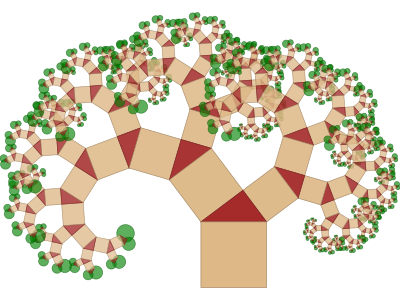
\includegraphics[width=0.235\textwidth]{html/PythagoreanTree.png}
\end{center}
%*endignore

Some other exciting recent things in diagrams-land:
\begin{itemize}
\item The \texttt{diagrams-builder} package allows rendering diagrams
  dynamically, at run time, and has been used to support things like
  inline diagrams code in blog posts and \LaTeX\ documents (see
  \url{https://byorgey.wordpress.com/2012/08/28/creating-documents-with-embedded-diagrams/}).
\item Brent recently presented a paper at the Haskell Symposium,
  \emph{Monoids: Theme and Variations}, based on diagrams and
  motivating the design of some of its core data structures:
  \url{http://www.cis.upenn.edu/~byorgey/pub/monoid-pearl.pdf}.
\end{itemize}

%**<img width=350 src="./FibCalls.png">
%*ignore
\begin{center}
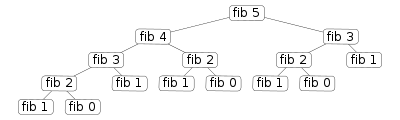
\includegraphics[width=0.33\textwidth]{html/FibCalls.png}
\end{center}
%*endignore

\subsubsection*{Contributing}

There is plenty of exciting work to be done; new contributors are
welcome!  Diagrams has developed an encouraging, responsive, and fun
developer community, and makes for a great opportunity to learn and
hack on some ``real-world'' Haskell code.  Because of its size,
generality, and enthusiastic embrace of advanced type system features,
diagrams can be intimidating to would-be users and contributors;
however, we are actively working on new documentation and resources to
help combat this.  For more information on ways to contribute and how
to get started, see the Contributing page on the diagrams wiki:
\url{http://haskell.org/haskellwiki/Diagrams/Contributing}.

%**<img width=500 src="./triangular-numbers.jpg">
%*ignore
\begin{center}
\includegraphics[width=0.47\textwidth]{html/triangular-numbers.jpg}
\end{center}
%*endignore

\FuturePlans

Some exciting work on animation, interactivity, and using diagrams as
a high-powered presentation tool is underway---stay tuned!

A native SVG backend is under active development and almost ready to
be used as a drop-in replacement for the cairo backend.  The cairo
backend will still be supported, but SVG will replace cairo as the
default ``out-of-the-box'' backend, vastly simplifying installation
for new useres. Other features planned for the near future include
better arrow support, multi-page diagrams, and gradients.  Longer-term
plans include a richer API for drawing curved paths, interactive
diagrams, and a custom Gtk application for interactively developing
diagrams and animations.

\FurtherReading
\begin{compactitem}
\item \url{http://projects.haskell.org/diagrams}
\item \url{http://projects.haskell.org/diagrams/gallery.html}
\item \url{http://haskell.org/haskellwiki/Diagrams}
\item \url{http://github.com/diagrams}
\item
  \url{https://byorgey.wordpress.com/2012/08/28/creating-documents-with-embedded-diagrams/}
\item \url{http://www.cis.upenn.edu/~byorgey/pub/monoid-pearl.pdf}
\item \url{http://www.youtube.com/watch?v=X-8NCkD2vOw}
\end{compactitem}
\end{hcarentry}
